%!TEX root = Nanomat.tex
\ctitle{Nanoskala vekst}
%\cstitle{Termodynamikk for faseoverganger}
\paragraph{En faseovergang kan være mye rart} Den typen faseovergang som de fleste er kjent med kan være en endring i aggregattilstand, for eksempel smelting (fast stoff til væske) eller kondensering (gass til væske). En faseovergang kan også være en endring i krystallstruktur, for eksempel fra en paramagnetisk til en ferromagnetisk struktur. En faseovergang kan også være separasjon av faser, for eksempel når en homogen blanding av to væsker skiller seg ut i to forskjellige faser.

%\paragraph{Landaus modell for faseoverganger} Den enkleste og mest generelle modellen for faseoverganger er Lev Landau sin. I Landaus modell brukes en ordningsparameter $\phi$. Hva $\phi$ representerer avhenger av hva slags faseovergang man har. I endring av aggregattilstand vil det være naturlig å la $\phi$ være materialets tetthet, siden endring i tetthet er det som karakteriserer en slik overgang. Når et materiale går fra å være paramagnetisk til å være ferromagnetisk, vil det være naturlig å heller la $\phi$ være verdien til magnetiseringen, siden dette er materialegenskapen som karakteriserer en slik overgang. Og i tilfellet med separasjon av faser vil det være naturlig å la $\phi$ være konsentrasjon (egentlig forskjellen i konsentrasjon mellom de to fasene).

%I Landaus modell uttrykkes den frie energien (egentlig den frie energitettheten) gjennom ordningsparameteren:
%\begin{equation}
%	\Delta f(\phi) = \Delta f_0 + \mu\Delta\phi + a\Delta\phi^2 + b\Delta\phi^4 + O(\Delta\phi^5)
%\end{equation}
%Hvis du lurer på hvor det ble av $\Delta\phi^3$, og generelt syntes at dette høres ut som en spennende ting å bruke mye tid på, så kan du lese s. 384-385 i Bréchnigac.\footnote{Ellers er det bare å glemme Landau og modellen hans. Du trenger den nemlig kun hvis du skal se på termodynamikken til spinodal dekomponering, men når vi kommer til spinodal dekomponering hopper vi over termodynamikken.}

\cstitle{Faseovergangers dynamikk}
En faseovergang vil ikke nødvendigvis forekomme selv om faseovergangen er termodynamisk foretrukket, og den vil uansett ikke skje umiddelbart. For å gjennomføre en faseovergang er det nødvendig at de kjemiske speciene faktisk beveger seg der de skal. Vi kan få dem til å gjøre dette ved å
\begin{itemize}
	\item Stadig tilføre reaktant. Dette tilfellet skal vi se nøye på i avsnittet om den Veldig Viktige Figuren.
	\item Senke temperaturen, slik at løseligheten også synker, og nanopartikler presipiterer ut av løsningen.
	\item Endre pH på en måte som senker løselighet.
	\item Blande to ioniske løsninger slik at det dannes et uløselig salt.
	\item Starte en kjemisk reaksjon som produserer uløselige specier.
\end{itemize}

Man har to typer mekanismer for faseoverganger. Den første, vanligste og viktigste (for oss) er nukleering og vekst, og den andre heter spinodal dekomponering.

\paragraph{Nukleering og vekst}
Nukleering og vekst begynner ved at små kim (også kjent som kjerner, også kjent som nuklei) av en ny fase oppstår spontant. Endringen i fri energi ved danelsen av et slikt kim er
\begin{equation}
	\label{eq:nucl_growth}
	\Delta G(r) = V(r)\Delta g_V + A(r)\gamma
\end{equation}
der $r$ er kimets radius, $\gamma$ er overflatespenning, og $\Delta g_V$ er forskjellen i fri-energi-tetthet mellom den nye og den gamle fasen.\footnote{I denne sammenhengen er det fristende å skrive $\gamma$ som $\Delta g_A$ for å få et mest mulig elegant uttrykk: $\Delta G=V\Delta g_V + A\Delta g_A$. Men $\gamma$ er det vanlige, så da holder vi oss til det.} $\Delta g_V$ må være negativ for at faseovergangen i det hele tatt skal være termodynamisk foretrukket.\footnote{Bréchnigac skriver det som ``$\Delta E(R) = -\Delta \mu R^3 + \gamma R^2$'', der minustegnet forteller at energien synker når den nye fasen dannes. Hvis vi ser bort i fra at symbolene ikke er forklart (hvis uttrykket skal gi mening, kan de i hvert fall ikke bety det de pleier å bety), så må man altså ha $\Delta \mu = \mu_{\text{før}} - \mu_{\text{etter}}$ for å få ligningen til å gå opp. Og da betyr $\Delta$ nøyaktig det omvendte av det $\Delta$-symbolet betyr i alle andre sammenhenger. Dette er ikke greit. Man kan ikke holde på sånn.} Ligningen uttrykker balansen mellom to drivkrefter:
\begin{itemize}
	\item Det første leddet kan tenkes på som et ``bulk''-ledd, og er drivkraften for dannelsen av den nye fasen.
	\item Det andre leddet kan tenkes på som et ``grenseflate''-ledd. Dette leddet uttrykker hvordan diffusjon av atomer vil motvirke det veldig skarpe skillet i konsentrasjon i grenseflaten mellom den gamle og den nye fasen. 
\end{itemize}
\vfill
Hvis vi antar at kimene er sfæriske, kan vi utvide $V(r)$ og $A(r)$ i ligning \eqref{eq:nucl_growth}:
\begin{equation}
	\label{eq:nucl_growth_explicit}
	\Delta G(r) = \frac{4\pi r^3}{3}\Delta g_V+4\pi r^2 \gamma,
\end{equation}
som er et tredjegradspolynom i $r$. Det ser slik ut:
\begin{figure}[H]
	\centering
	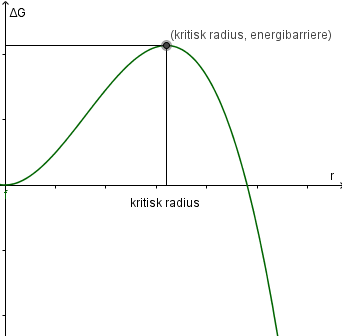
\includegraphics[width=\linewidth]{nucl.png}
	\label{fig:nucl}
\end{figure}
Figuren viser at man har en \emph{kritisk radius} $r_c$. Hvis kimet med den nye fasen klarer å få en radius større enn $r_c$, vil det være gunstig at det fortsetter å øke i størrelse, da dette får $\Delta G(r)$ til å synke. Hvis kimet ikke har klart å bli så stort, vil det være gunstig at det minker i størrelse og til slutt forsvinner. Den frie energien til et kim med radius $r_c$ blir dermed en energibarriere som kimene må overkomme for å vokse seg store. Siden den kritiske radien er ved toppunktet for $\Delta G(r)$ kan vi finne den som vi gjorte i Matte 1 (sett den deriverte lik null) for å få at
\begin{equation}
	r_c=-\frac{2\gamma}{\Delta g_V},
\end{equation}
og at energibarrieren assosiert med denne radien er
\begin{equation}
	\Delta G_c = \frac{16\pi\gamma^3}{3(\Delta g_V)^2}.
\end{equation}

\paragraph{En Veldig Viktig Figur} Her er en figur. Denne figuren må du kunne. Denne figuren er så viktig at jeg har kalt den ``den_veldig_viktige_figuren.png''. Du må vite hva alle tallene i denne figuren representerer.
\begin{figure}[H]
	\centering
	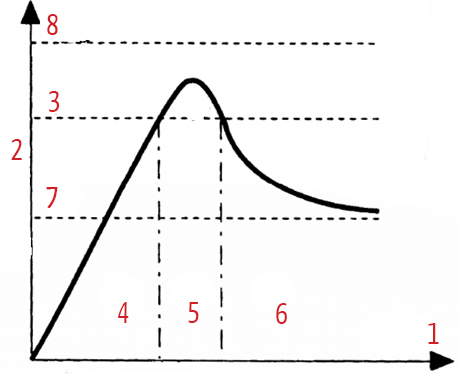
\includegraphics[width=\linewidth]{den_veldig_viktige_figuren.png}
	\label{fig:viktig}
\end{figure}
Her er fasit:
\begin{enumerate}
	\item $x$-aksen er tid. Eller, det er egentlig et slags reaksjonskoordinat i en prosess der man kontinuerlig tilfører reaktantene som trengs for å gjennomføre faseovergangen.
	\item $y$-aksen er konsentrasjonen av reaktanten som trengs for å gjennomføre faseovergangen (det står ``solute concentration'' på den opprinnelige figuren). Denne konsentrasjonen inkluderer \emph{ikke} det som er i kimene.
	\item Denne stiplede linjen representerer en konsentrasjon $C_{\text{min}}^{\text{nukl.}}$. Dette er minimumskonsentrasjonen for at det skal presipiteres partikler. Sagt på en annen måte: det er metningsevnen til løsningen.
	\item Dette er trinn I i prosessen. Det tilføres reaktant, og konsentrasjonen av reaktanten i løsningen øker stadig. Av og til dannes det kim, men disse er for små til å være stabile, så de oppløses raskt tilbake i løsningen.
	\item Dette er trinn II i prosessen, nemlig nukleering og vekst. Det begynner nå å dannes kim som kan bli stabile og vokse. Nukleeringsraten eksploderer når konsentrasjonen passerer $C_{\text{min}}^{\text{nukl.}}$, så det tar ikke lang tid før nukleeringen skjer så raskt at konsentrasjonen av reaktant i løsningen går \emph{ned}, selv om vi stadig tilfører mer reaktant.
	\item Dette er trinn III i prosessen, nemlig vekst. I dette trinnet har konsentrasjonen falt under $C_{\text{min}}^{\text{nukl.}}$, så nye kim som oppstår er ikke stabile og oppløses raskt tilbake i løsningen. Forskjellen mellom trinn I og trinn III er at vi nå har en masse stabile kim i løsningen.
	\item Løsningen når etter hvert en likevektskonsentrasjon, $C_s$ på grunn av entropi og sånn.
	\item Denne stiplede linjen representerer en konsentrasjon $C_{\text{max}}^{\text{nukl.}}$. Jeg aner ikke hva som er poenget med den, men den har åpenbart ikke noen innvirkning på prosessen.
\end{enumerate}

\paragraph{Agglomerering og Oswald ripening} Mens kimene vokser skjer også en annen effekt: forskjellige kim begynner å feste seg til hverandre og smelte sammen i en prosess som kalles agglomerering.\footnote{Hvis du vil være fancy kan du si at sammensmelting ved dannelse av svake bindinger er agglomerering, og sammensmelting ved dannelse av sterke bindinger er aggregering. Folk blander dem sammen så ofte at noen faktisk måtte sette seg ned og skrive en artikkel som heter``A review of the terms agglomerate and aggregate with a recommendation for nomenclature used in powder and particle characterization''. Det virker som om ``agglomerering'' er et mer generelt begrep enn alternativet, så da går vi for det.} Gjennom agglomerering samler kimene seg sammen til det som i det endelige produktet blir kornene i materialet.

Det har seg slik at store kim ``spiser opp'' mindre kim de kommer i kontakt med. Dette fenomenet kalles Oswald ripening.

Merk at både agglomerering og Oswald ripening kan fortsette etter at selve veksten har opphørt.

\paragraph{Homogen og heterogen nukleering} Hvis man begynner med en helt homogen løsning, må man få den tilfeldige termiske energien til å dytte sammen partikler på riktig måte slik at det spontant oppstår kim som er store nok. Det innebærer en ganske stor energibarriere. For å få til dette må man lage en supermettet løsning, altså kjøre konsentrasjonen av reaktant ganske langt forbi den egentlige løseligheten til reaktanten i løsemiddelet.

Hvis man har forurensninger, suspenderte partikler eller små bobler i løsningen blir det hele mye enklere. Det blir som å allerede ha ``ferdige'' kim i løsningen, som den nye fasen kan vokse på. Dette gjør energibarrieren betraktelig mindre.\footnote{Fin MinuteEarth-video: https://www.youtube.com/watch?v=87v_9Bud7vw}

% Smal fordeling av størrelser = rask nukleering, bred fordeling = treg nukleering

% Homogen og heterogen nukleering: kjent. Husk at suspenderte partikler eller små bobler også er nucleation sites og gjør det til heterogen nukleering. Se/forklar graf

\paragraph{Spinodal dekomponering}
\label{sec:spinodal_decomposition}
Spinodal dekomponering er når en løsning av to eller flere komponenter separerer seg i distinkte regioner eller faser med distinkte kjemiske og fysiske egenskaper, spontant gjennom hele materialet og uten en aktiveringsbarriere. Det er altså ganske annerledes fra nukleering og vekst. Resultatet av spinodal dekomponering ser typisk litt sånn ut:
\begin{figure}[H]
	\centering
	
\includegraphics[width=\linewidth]{spino.png}
	\label{fig:spino}
\end{figure}
Spinodal dekomponering finner vi ofte i løsninger av to faste metaller, og i glassmaterialer.

\cstitle{Størrelseskontroll}
I både nukleering-vekst og spinodal dekomponering er de første strukturene som oppstår, noen nanometer store. Siden vi skal lage nanomaterialer er vi interessert i å beholde disse små strukturene og hindre at de vokser seg større.

\paragraph{Hvordan får vi en smal fordeling av størrelser i det endelige produktet?} Vi må få så mye av nukleeringen som mulig til å skje samtidig, og deretter bør nukleeringen raskt opphøre.\footnote{Lurer på hvordan vi sørger for det. På sliden står det bare ``A simple mixture usually leads to large concentration
gradients and hence to a large size distribution of particles. How do we avoid this?'' og ikke noe mer.}

\paragraph{Hvordan sørger vi for at kimene vokser til den størrelsen vi ønsker oss, men ikke videre?} Siden vekst skjer ved at atomer/molekyler fra løsningen diffunderer bort til partiklene, kan vi hindre veksten ved å putte noe mellom løsningen og partiklene. Hvis vi lager titanoksid-partikler kan vi introdusere ``complexing agents'' som acetylaceton eller eddiksyre, som danner komplekser med partiklene og blokkerer molekylene fra løsningen. Man kan også bruke \emph{mineraliserende agenter}, for eksempel fluorid, som for eksempel kan tilføres reaksjonen i form av et salt. Hvis disse fester seg på overflaten av kimene, vil det hindre dem fra å vokse videre.

\paragraph{Hvordan forhindrer vi agglomerering?} For å hindre at kimene fester seg til hverandre kan vi introdusere energibarriere som blir uoverkommelig når partiklene når en viss størrelse. Det finnes to generelle metoder for å introdusere denne barrieren:
\begin{itemize}
	\item Elektrostatisk stabilisering: hvis reaksjonen skjer i vannløsning, kan man prøve å få overflaten til å danne en elektrisk ladning, for eksempel ved at det adsorberes ioner i mediet. Dette hindrer ikke vekst, men frastøtning mellom partiklene hindrer dem fra å aggregere eller smelte sammen. 
	\item Sterisk stabilisering: vi kan la det adsorberes polymerer, proteiner eller surfaktanter på overflaten av partiklene. Sterisk hindring mellom disse adsorberte molekylene hindrer partiklene fra å komme nærmere hverandre enn ca. lengden til molekylet.
\end{itemize}
